\documentclass[12pt]{article}
\usepackage[utf8]{inputenc}
\usepackage{cleveref}
\usepackage{graphicx}
\usepackage{subfig}
\usepackage{geometry}
\usepackage{bbm}
\usepackage{amsmath}
\usepackage{algpseudocode}
\usepackage{hyperref}
\usepackage{amsthm}
\usepackage{xcolor}

\DeclareMathOperator*{\argmin}{arg\,min}
\geometry{a4paper, left=30mm, right=30mm}

\setlength\parindent{0pt}
\newcommand{\R}{\mathbbm{R}}
\newcommand{\1}{\mathbbm{1}}
\newcommand\note[1]{\textcolor{red}{\textbf{#1}}}
\newtheorem{theorem}{Theorem}


\title{Conjugate Gradient for \\ Quadratic Minimum-Cost Flow}
\author{Lorenzo Beretta, \texttt{loribere@gmail.com}
  \and Project NoML-13 of C.M. course, C.S. department, UniPi}
\date{3rd July 2019}

\begin{document}
\maketitle


\section{Introduction}
Let $D \in {\R^{m \times m}$ be a diagonal positive definite matrix and $E \in \R^{n \times m}$ be the node-edge matrix of a directed graph, meaning that, given an enumeration $e[1\dots m]$ of edges, we have
  \begin{equation*}
    E_{i, j} = \left\{
      \begin{align*}
        1 \qquad&  \text{ if $e[j] = (u, v)$ and $j = v$} \\
        -1 \qquad& \text{ if $e[j] = (u, v)$ and $j = u$} \\
        0 \qquad&  \text{ otherwise}
      \end{align*}
   \end{equation*}
        
The aim of this project is to exploit the Conjugate Gradient method to solve the
linear system

\begin{equation} \label{linear_system}
  \left(E D^{-1} E^t\right) x = b
\end{equation}

for some $b \in \R^n$. 

This problem arises from the KKT conditions of a quadratic separable Minimum-Cost
Flow problem, however we will neglect its origin and just deal with the linear system.


\section{Conjugate Gradient Algorithm}
In this section we will show the conjugate gradient method to solve a linear  system of the form $ A x = b $ for a symmetric and positive semidefinite matrix $A$.

Our main reference for this method is the book of Trefethen {\em et al.} \cite{trefethen97} that treats the strictly positive definite case, it is easy to adapt their proofs to show that assuming $b \in range(A)$ all results stated there hold even in the semidefinite case. This is necessary to our application since $E^t D^{-1} E$ has rank exactly $n-1$ in fact $rk(E)=n-c$ where $c$ is the number of connected components of the graph (assumed to be connected) and $rk(D) = m$.
Of course the algorithm converges to one of the infinite solutions of the system if $rk(A) < n$ and in particular it converges to $x_*$ such that $\1^t x_* = 0$, indeed $Ker(E^t D^{-1} E) = \langle \1 \rangle$.

\subsection{Algorithm}
In the following algorithm $x_n$ is the approximate solution at step $n$ and the cycle is actually repeated until a suitable convergence error is achieved\footnote{In our implementation we emulated the scipy's CG criterion, stopping as soon as $\frac{||r_n||_2}{ ||b||_2}$ falls below a fixed threshold.}.

\vbox{
\begin{algorithmic}[1]
\Procedure{ConjugateGradient}{$A, b$}
  \State {$ x_0 = 0, \quad r_0 = b, \quad p_0 = b $}
  \For {$ n = 1,\, 2,\, 3,\, \dots $}
    \State {$ \alpha_n = \left(r_ {n-1}^tr_ {n-1}\right) / \left(p_ {n-1}^tAp_ {n-1}}\right) $} \Comment{Step Length}
    \State {$ x_n = x_{n-1} + \alpha_n p_{n-1} $} \Comment{Approximate Solution}
    \State {$ r_n = r_{n-1} - \alpha_n A p_{n-1} $} \Comment{Residual}
    \State {$\beta_n = \left(r_n^t r_n\right) / \left(r_{n-1}^t r_{n-1}^t\right)$} \Comment{Improvement this Step}
    \State {$p_n = r_n + \beta_n p_{n-1} $} \Comment{Search Direction}
  \EndFor
\EndProcedure
\end{algorithmic}
}
\hspace{1cm}

It is worth noting that the bottleneck of the single iteration is the computation of $Ap_{n-1}$ and it can be fasten up considering the structure of A. It suffices to notice that $E$ has exactly $2m$ nonzero elements and employ a sparse matrix multiplication to achieve an $O(m)$ complexity per iteration. Moreover our implementation performs exactly $m$ multiplications and $3m$ additions keeping the constant factor very low\footnote{See \texttt{make\_operator} method in \texttt{cg.py} for more details.}.

\subsection{CG as a Direct Method}
The main property of this algorithm is that for every $n$ such that the algorithm has not converged yet it holds that:

\begin{equation*}
  \mathcal{K}_n = \langle x_1,\, \dots,\,x_n\rangle = \langle r_0,\, \dots,\,r_{n-1}\rangle = \langle p_0,\, \dots,\,p_{n-1}\rangle = \langle b,\,A b, \, \dots,\,A^{n-1} b\rangle \\
\end{equation*}

\begin{equation*}
  r_n^t r_j = 0, \quad p_n^t A p_j = 0 \quad \forall j < n
\end{equation*}
\hspace{0.5cm}

It is easy to show that this property entails that the algorithm is well defined even in the singular case since $ b \in range(A) \implies p_{n-1} \in range(A) \implies p_{n-1}^t A p_{n-1} \neq 0$. Moreover the fundamental corollary of that property is that  at each step
$$x_n = \argmin_{z \in \mathcal{K}_n} || x_* - z ||_A $$
for every $x_*$ such that $Ax_* = b$. Therefore in exact arithmetic it must converge in at most $n$ steps and the method is then a direct one.

\subsection{CG as an Interative Method}
Conjugate gradient has a twofold nature and can be interpreted as an optimization algorithm whose objective function is $ || x_* - x ||_A $ that up to a positive scaling and a shift is equal to $ \frac{1}{2}x^t A x - x^t b$. Then it becomes interesting to study its convergence rate trying to speedup the direct method bound of $n$ iterations.

The main result employed to derive the convergence rate is this slight modification of theorem 38.3 of Trefethen {\em et al.} \cite{trefethen97}:

\begin{theorem}[Polynomial Approximation]\label{polap}
  Let us define $e_n = x_* - x_n$ and $P_n = \left\{p \in \R[x]\, |\, deg(p) \leq n, \; p(0) = 1 \right\}$. If CG is not converged yet before step $n$ (i.e. $r_{n-1} \neq 0$) then 
$$ \frac{||e_n||_A}{||e_0||_A} \leq \inf_{p \in P_n}\frac{||p(A) e_0||_A}{||e_0||_A} \leq \inf_{p \in P_n} \max_{\lambda \in sp(A)\setminus\{0\}}|p(\lambda)|
$$
\end{theorem}
\begin{proof}
  Let us decompose $e_0$ over the orthonormal basis of $A$-eigenvectors as\\ $e_0 = \sum_i a_i v_i$ provided that $A v_i = \lambda_i v_i$, then
$$\inf_{p \in P_n}\frac{||p(A) e_0||_A}{||e_0||_A} \leq \inf_{p \in P_n}\sqrt{\frac{\sum_i a_i^2 \lambda_i \left(p(\lambda_i)\right)^2}{\sum_i a_i^2 \lambda_i}}\leq \inf_{p \in P_n} \max_{\lambda \in sp(A)\setminus\{0\}}|p(\lambda)|$$

\end{proof}

 Theorem \ref{polap} enhances theorem 38.3 of Trefethen {\em et al.} \cite{trefethen97} taking into account the singular case and showing that even in that case this bound doesn't degrade.

\subsection{Rate of Convergence}
The results above provide a better although trivial estimate for the ``exact method'' convergence time, in fact if $A$ has $h$ nonzero different eigenvalues then after $h$ iterations RHS in the previous inequality is null since the polynomial perfectly interpolates them.

On the other hand a more technical result involving the iterative nature of the algorithm can be proven: given $A$'s condition number $\kappa = \frac{\lambda_{max}}{\lambda_{min}}$, where $\lambda_{max}$ and $\lambda_{min}$ are extremal eigenvalues, it holds that

$$ \frac{||e_n||_A}{||e_0||_A} \leq 2 \left(\frac{\sqrt{\kappa} - 1}{\sqrt{\kappa} + 1}\right)^n $$

Finally we may say that a ``good'' spectrum for $A$ (i.e. providing fast convergence of CG) is one that has at least one of the two: (i) eigenvalue forms small clusters so that polynomials can interpolate them ``all at once'' or (ii) eigenvalues are not too separated in logarithmic scale. We will assess a strong dependence of convergence time on eigenvalues distribution experimentally. 


\section{Experiments}
In this section we will describe a series of experiments challenging our implementation of CG feeding it with a dataset tailored to push it to the theoretical limits proven so far. We will first describe how to generate the dataset, then we will deal with a tough question: how does $D \mapsto E^t D^{-1} E$ affect eigenvalues distribution? Finally we will show that our implementation works and compare it with off-the-shelf sparse linear solvers with and without precondition.

\subsection{Data Generation}
In order to perform the experiments we needed to generate three objects: the matrix $E\in \R^{n\times m}$ (equivalent to generate a digraph's topology), the diagonal positive definite matrix $D\in\R^{m\times m$ and the vector $b\in\R^n$.
  
As far as network generation is concerned we used the standard MCF instance generator \texttt{netgen}\footnote{See Klingman {\em et al.} \cite{netgen}} retrieved at \href{https://github.com/emmanuj/netgen}{https://github.com/emmanuj/netgen} as a C version.
This generator made it possible to vary number of nodes and arc density so that we could test our algorithm over several examples.

Since eigenvalues distribution plays a key role in iterative algorithms' convergence rate and, as stated in the previous section, this holds especially for CG, we deemed the distribution of $D$-eigenvalues as a critical parameter to study experimentally. Trying to figure out a meaningful parametrized distribution to sample from we found that, given the CG convergence rate as a function of $\kappa =  \frac{\lambda_{max}}{\lambda_{min}}$ it would have been nice to have $E^t D^{-1} E$ eigenvalues $0$-symmetrically distributed in logarithmic scale. Although the distribution of $E^t D^{-1} E$ eigenvalues cannot be simply inferred form the one of $D$ (we will see this later in more details) we opted for sampling $D$'s entries exponentiating a r.v. uniformly distributed over $[-rad_D, rad_D]$.  

Finally we needed to generate $b$ such that $\1^t b = 0$ so we just sampled each of $b$'s entries uniformly from an interval $[-rad_b, rad_b]$ and then subtracted from $b$ its projection on $\langle \1 \rangle$. We will see through experiments that $rad_b$ value does not affect our algorithm's performance. 

\subsection{Eigenvalues Distribution}
To grasp some informations about how does $E^t D^{-1} E$ eigenvalues vary while tuning $rad_D$ and the arc density of graph, we plotted the eigenvalues\footnote{Calculated with \texttt{numpy.linalg.eigvals}.} of a $100 \times 100$ matrix induced by a $100$-nodes graph generated as stated above. Please notice that eigenvalues' norm are in logarithmic scale.

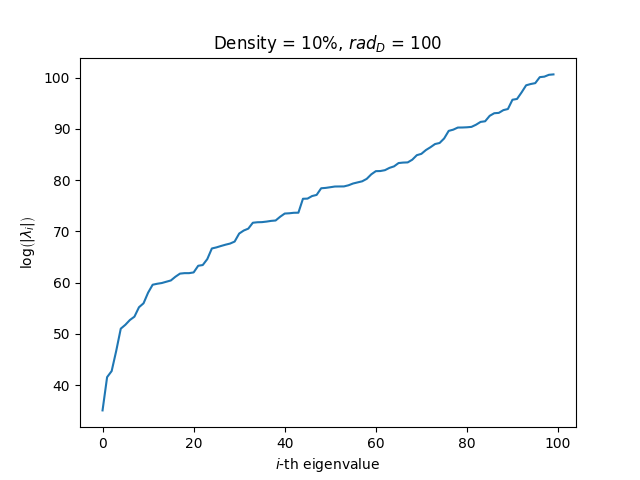
\includegraphics[scale=0.5, H]{eigen-100-10-100.png}
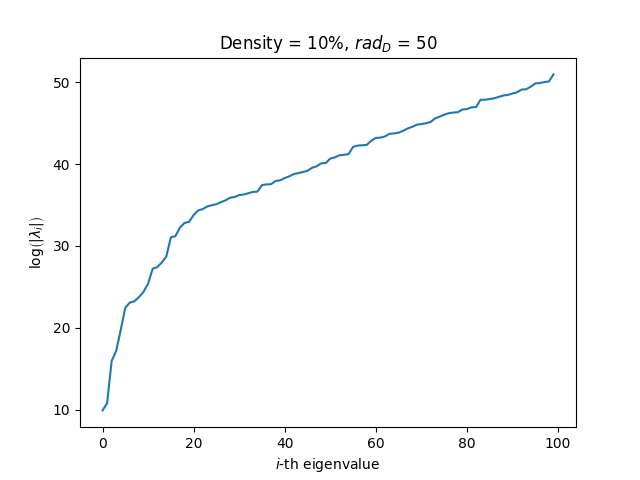
\includegraphics[scale=0.5, H]{eigen-100-10-50.png}
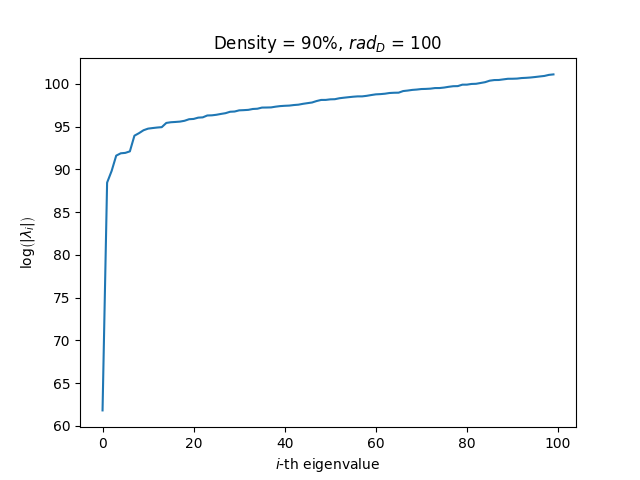
\includegraphics[scale=0.5, H]{eigen-100-90-100.png}
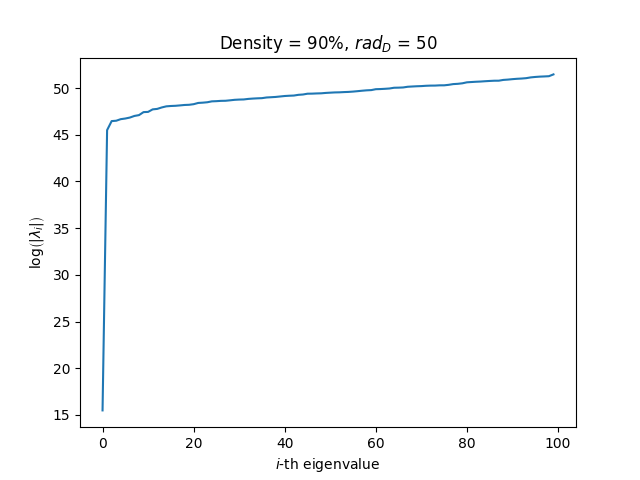
\includegraphics[scale=0.5, H]{eigen-100-90-50.png}

As you can see the matrices in the first row, having 10\% arc density, present much more evenly distributed eigenvalues and then we expect CG to have worse convergence on them. As we could easily expect widening up $rad_D$ condition number get worse. We will take this into account later employing a proper precondition while dealing with such matrices.  

\subsection{CG Implementation Performance}
From now on we will show results of experiments consisting of iterative methods solving linear systems, then our main benchmark parameters will be the number of iteration and the time elapsed (experiments have been run on a single machine
\footnote{Intel i3-6006U CPU, x86\_64, 2.00GHz running Linux Debian 9.}). In order to make different solvers comparable we set a uniform stopping criterion halting the iteration loop as soon as the residual norm divided by $||b||_2$ falls below a fixed amount (default is $1e-05$).

Let us start with a couple of plots showing that our implementation works: the first one took 10.1 \textit{seconds} and achieved a relative error $\left(\text{i.e.} \frac{||Ax - b||_2}{||b||_2}\right)$ of 8.3e-06 while the second took 16.2 \textit{seconds} attaining 8.9e-06 as relative error. 

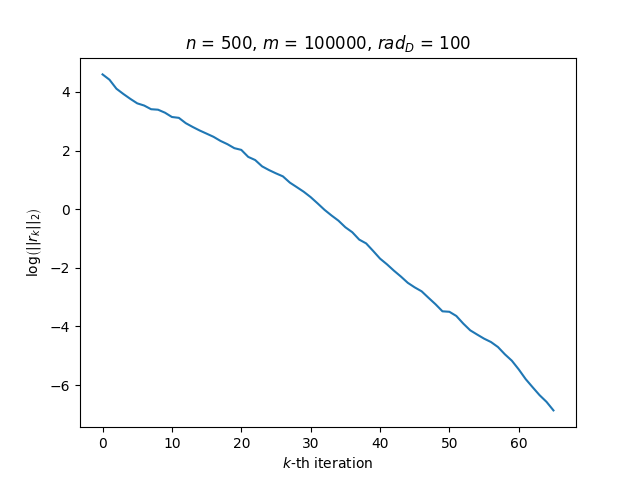
\includegraphics[scale=0.5, H]{my_cg-500-100000-100.png}
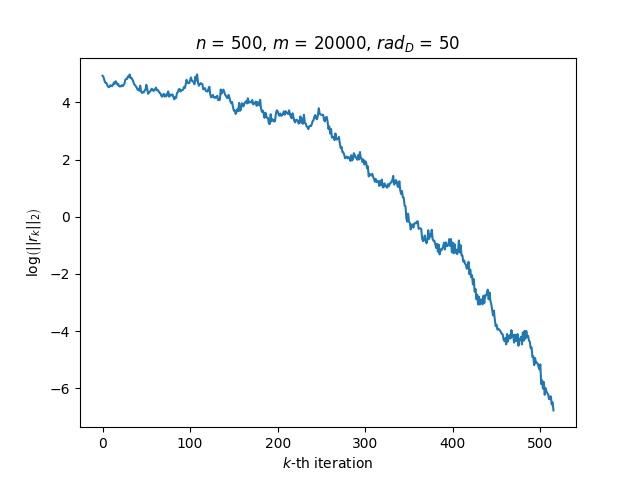
\includegraphics[scale=0.5, H]{my_cg-500-20000-50.png}

It is worth noting that, even if the former graph has both a twice wider $rad_D$ and 5 times more arcs than the latter, CG is clearly faster on the former both in terms of iterations and elapsed time. This is due, of course, to eigenvalues that, as showed above, are much more evenly distributed
when the graph is dense preventing the polynomials of Theorem \ref{polap} to closely interpolate them. 

In the following tables we report more experiments conducted on \texttt{my\_cg}, our own implementation of CG. We will vary one of $n$, $m$ and $rad_D$ at a time keeping the others fixed.

\begin{center}
  \vbox{
 $n = 300$, $rad_D = 100$ :\\
    \begin{tabular}{| l | l | l | l | l |}
      \hline
      $m =$       & 1500   & 20000  & 25000   & 40000  \\
      \hline
      \hline
      Iterazioni  & 1290   & 457    & 357   & 93  \\
      \hline    
      Tempo       & 31.5 s & 14.8 s & 14.2 s & 5.8 s  \\
       \hline    
    \end{tabular}}
\end{center}
\begin{center}
  \vbox{
 $rad_D = 100$, $m = 20000$ :\\
    \begin{tabular}{| l | l | l | l | l |}
      \hline
      $n =$  & 150   & 200   & 300    & 400  \\
      \hline
      \hline
      Iterazioni  & 81    & 139   & 548    & 1283   \\
      \hline    
      Tempo       & 2.7 s & 9.4 s & 20.1 s & 46.3 s  \\
       \hline    
    \end{tabular}}
\end{center}
\begin{center}
  \vbox{
 $n = 250$, $m = 20000$ :\\
    \begin{tabular}{| l | l | l | l | l |}
      \hline
      $rad_D =$  & 50   & 75 & 100   & 150  \\
      \hline
      \hline
      Iterazioni  & 92   & 177  & 309   & 730   \\
      \hline    
      Tempo       & 2.9 s & 5.6 s & 10.2 s & 24.8 s  \\
       \hline    
    \end{tabular}}
\end{center}

Again these data show that the sparser is the graph the slower is CG, in fact adding arcs fasten up the algorithm significantly. Moreover as expected sampling $D$'s entries from a wider interval yields a worse conditioned matrix and then a slower CG. Once sen the first two tables the third one is not very surprising, indeed augmenting $n$ not only make the graph sparser but increases the size of linear system.  

\subsection{Distribution of $b$}
As stated in the theoretical part of this report, the choice of $b$ does not affect the convergence rate. Although it could be a legit question to ask whether the choice of $b$ significantly impacts the number of iteration or elapsed time. We will briefly show experimentally that this is not the case and that we do not need to bother with its distribution while comparing methods.

In the following experiment we will sample $b$'s entries uniformly from $[-rad_b, rad_b]$ and then orthogonalize it with respect to $\1$. We will show that CG performance is independent from $rad_b$.

\begin{center}
  \vbox{
 $n = 200$, $m = 20000$, $rad_D = 100$ :\\
    \begin{tabular}{| l | l | l | l | l |}
      \hline
      $rad_b =$  & 1   & 10 & 100   & 1000  \\
      \hline
      \hline
      Iterazioni  & 126   & 129  & 119   & 130   \\
      \hline    
      Tempo       & 5.8 s & 6.2 s & 5.4 s & 5.7 s  \\
      \hline    
    \end{tabular}}
\end{center}


\subsection{Preconditioning}
When $E^t D^{-1} E$ is too ill conditioned to be dealt with it is a good strategy to try to find a matrix $M$ such that $M y = c$ is easily solvable and $M^{-1}A$ is less ill conditioned than $A$.
It is reasonable\footnote{According to Demmel\cite{demmel}.}, if diagonal entries vary a lot, to employ the Jacobi preconditioner that is to define $M = diag(A)$.

To show that diagonal entries actually vary a lot let us plot their norm for a matrix $A$ generated from a sparse graph, in particular setting $n = 100$, $m = 500$ and $rad_D = 50$.
\begin{center}
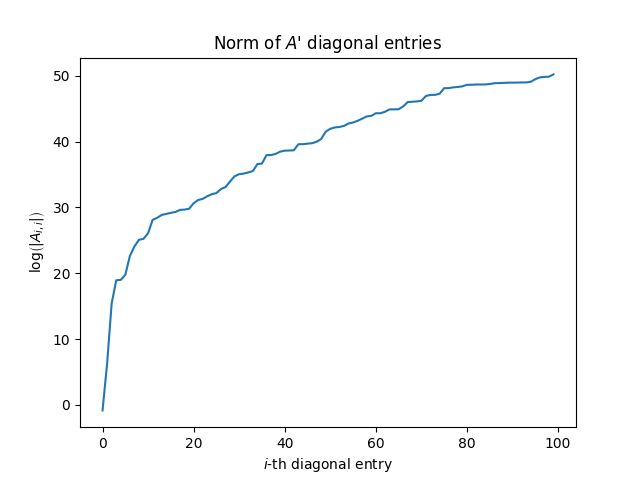
\includegraphics[scale=0.7, H]{diag-100-500-50.png}
\end{center}

In the following experiments we employed Jacobi preconditioner to improve CG speed. We kept $n = 100$ and $rad_D = 50$ constant and let $m$ vary\footnote{We were not able to compare the algorithms applied on the plotted matrix (i.e. $m=500$) since just the preconditioned one terminates on such a ill conditioned matrix.} so that we are able to notice again the effect of sparsity on conditioning and how precondition deals successfully with that.

\begin{center}
\begin{minipage}{0.45\textwidth}
  \vbox{
 Non-Preconditioned :\\
    \begin{tabular}{| l | l | l | l | l |}
      \hline
      $m =$  & 1000   & 1500 & 4000  \\
      \hline
      \hline
      Iterazioni  & 2383   & 498  & 122    \\
      \hline    
      Tempo       & 3.7 s & 1.2 s & 0.9 s   \\
       \hline    
    \end{tabular}}
\end{minipage}
\begin{minipage}{0.45\textwidth}
  \vbox{
Preconditioned :\\
    \begin{tabular}{| l | l | l | l | l |}
      \hline
      $m =$  & 1000   & 1500 & 4000  \\
      \hline
      \hline
      Iterazioni  & 111   & 80  & 35    \\
      \hline    
      Tempo       & 0.3 s & 0.3 s & 0.3 s   \\
      \hline    
    \end{tabular}}
\end{minipage}
\end{center}


Then we repeated the experiment setting $n = 100$, $m = 4000$ and letting $rad_D$ vary in order increase progressively the condition number.

\begin{center}
\begin{minipage}{0.45\textwidth}
  \vbox{
 Non-Preconditioned :\\
    \begin{tabular}{| l | l | l | l | l |}
      \hline
      $rad_D =$  & 100   & 150 & 200  \\
      \hline
      \hline
      Iterazioni  & 281   & 455  & 1804    \\
      \hline    
      Tempo       & 1.9 s & 2.8 s & 12.7 s   \\
       \hline    
    \end{tabular}}
\end{minipage}
\begin{minipage}{0.45\textwidth}
  \vbox{
Preconditioned :\\
    \begin{tabular}{| l | l | l | l | l |}
      \hline
      $rad_D =$  & 100   & 150 & 200  \\
      \hline
      \hline
      Iterazioni  & 84   & 78  & 116    \\
      \hline    
      Tempo       & 0.7 s & 0.7 s & 1.1 s   \\
      \hline    
    \end{tabular}}
\end{minipage}
\end{center}

Finally this is a logarithmic scale plot of residual per iteration comparing preconditioned (yellow) and non-preconditioned (blue) CG over a matrix originated from a sparse graph:

\begin{center}
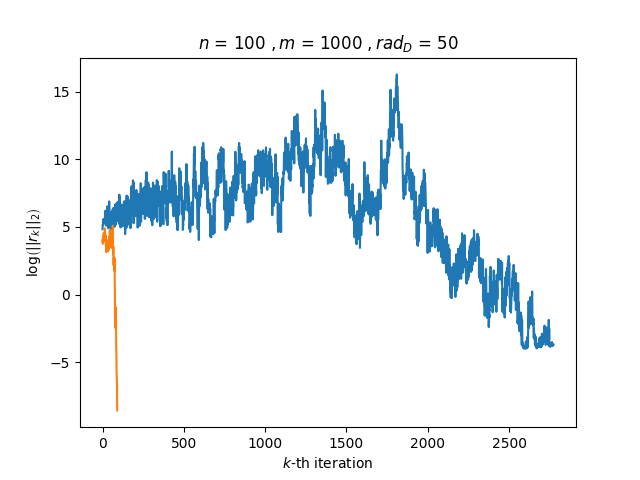
\includegraphics[scale=0.7, H]{prec-or-not.png}
\end{center}

\subsection{Off-the-Shelf Solver Comparison}
In this section we will compare our implementation of CG with an off-the-shelf solver from \texttt{scipy}: \texttt{gmres} a sparse linear system solver that implement the well known GMRES algorithm. Again we should take care that the stopping criterion makes the comparison fair, even though we set the same tolerance factor for both algorithms, it is not sufficient to guarantee fairness since they calculate residuals in different ways. However it is possible to ensure fairness through  an a posteriori assessment of their relative precision $\left(\text{i.e.} \frac{||Ax - b||_2}{||b||_2}\right)$ revealing that \texttt{my\_cg} is more precise (10\% on average) and that it is sufficient to prove that \texttt{my\_cg} outperforms \texttt{gmres}.

Let us compare \texttt{my\_cg} with \texttt{gmres} fixing the topology, we will keep $n = 500$ and $m = 100000$ and move $rad_D$.

\begin{center}
\begin{minipage}{0.45\textwidth}
  \vbox{
 \texttt{my\_cg} :\\
    \begin{tabular}{| l | l | l | l | l |}
      \hline
      $rad_D =$  & 50 & 100   & 150  \\
      \hline
      \hline
      Iterazioni  & 39   & 72  & 131    \\
      \hline    
      Tempo       & 5.8 s & 10.9 s & 20.2 s   \\
       \hline    
    \end{tabular}}
\end{minipage}
\begin{minipage}{0.45\textwidth}
  \vbox{
\texttt{gmres} :\\
    \begin{tabular}{| l | l | l | l | l |}
      \hline
      $rad_D =$  & 50 & 100   & 150  \\
      \hline
      \hline
      Iterazioni  & 50   & 150  & 275    \\
      \hline    
      Tempo       & 5.5 s & 16.1 s & 29.8 s   \\
      \hline    
    \end{tabular}}
\end{minipage}
\end{center}

CG outperforms GMRES both in time and number of iterations, especially when the matrix get more and more ill conditioned. Let us now vary $m$ fixing other parameters.


\begin{center}
\begin{minipage}{0.45\textwidth}
  \vbox{
 \texttt{my\_cg} :\\
    \begin{tabular}{| l | l | l | l | l |}
      \hline
      $m =$  & 30000 & 50000   & 100000  \\
      \hline
      \hline
      Iterazioni  & 153   & 53  & 26    \\
      \hline    
      Tempo       & 8.4 s & 4.1 s & 3.9 s   \\
       \hline    
    \end{tabular}}
\end{minipage}
\begin{minipage}{0.45\textwidth}
  \vbox{
\texttt{gmres} :\\
    \begin{tabular}{| l | l | l | l | l |}
      \hline
      $rad_D =$  & 30000 & 50000   & 100000  \\
      \hline
      \hline
      Iterazioni  & 356   & 79  & 27    \\
      \hline    
      Tempo       & 11.5 s & 4.3 s & 7.6 s   \\
      \hline    
    \end{tabular}}
\end{minipage}
\end{center}

Again it turns out that GMRES stays competitive as far as the matrix is well conditioned, but as soon as things get nastier CG prevails.

\section{Code}
The algorithm has been coded in \texttt{python 3.5} exploiting \texttt{scipy}, \texttt{numpy} and \texttt{matplotlib} libraries. Source code is well documented and it has been developed coherently with the \texttt{scipy} style so that \texttt{my\_cg} method has almost the same signature as the off-the-shelf solver and then they may be interchanged most of the time. All the core functions are in \texttt{cg.py} while \texttt{script.py} contains only methods to automate experimentation.
  
\bibliographystyle{acm}  
\bibliography{biblio}
\end{document}

%%% Local Variables:
%%% mode: latex
%%% TeX-master: t
%%% End:
